\subsection{Risposta dello spettrometro}

\paragraph{Stabilità} Facciamo una misura lunga circa 20 ore con la sorgente a \SI{70}{\degree} senza bersaglio per valutare la stabilità in risposta dello spettrometro (ovvero il sistema rivelatore-preampli-ampli-ADC).
La scelta dell'angolo è forzata dal rate di campionamento massimo (\SI{40}{Hz}) dell'ADC.

Mostriamo in \autoref{stab} i valori campionati in funzione del tempo.
Non osserviamo nessuna scalibrazione.

\begin{figure}[h]
\centering
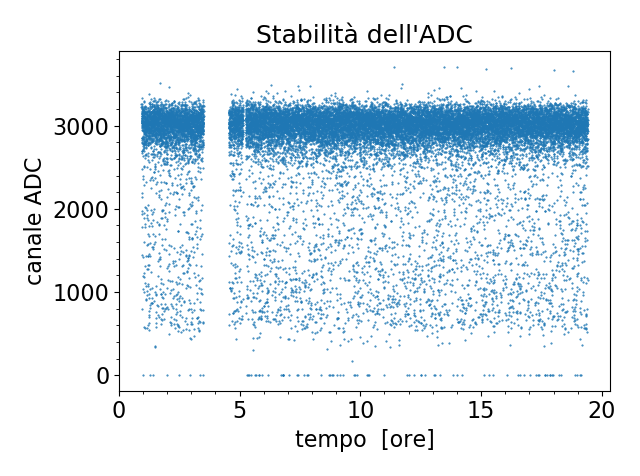
\includegraphics[width=23 em]{immagini/stab.png}
\caption{Valori acquisiti in funzione del tempo. Gli spazi vuoti tra una serie di dati e l'altra vengono dal fatto che sono state unite 4 acquisizioni quasi consecutive.
In questo grafico è presente soltanto un punto ogni 100 perché la rappresentazione completa rendeva illeggibile la figura.}
\label{stab}
\end{figure}

\paragraph{Forma dello spettro}

A titolo di esempio in \autoref{fig:example}
riportiamo lo spettro completo della presa dati per la verifica di stabilità.

\begin{figure}
	\centering
	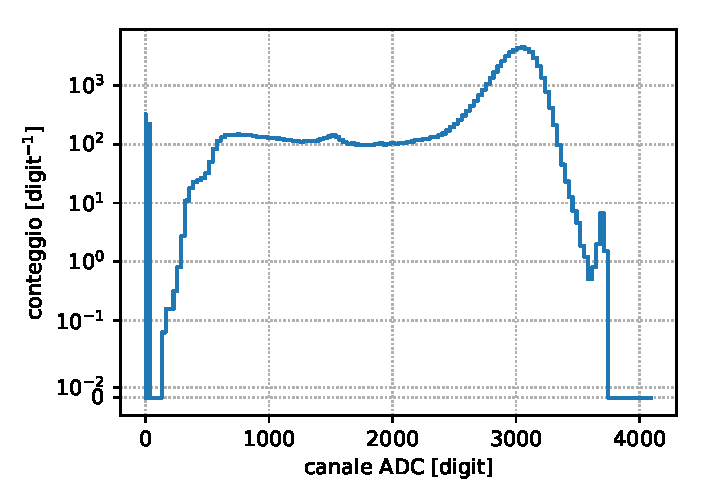
\includegraphics[width=25em]{immagini/example}
	\caption{\label{fig:example}
	Spettro senza bersaglio preso durante la notte.}
\end{figure}

\paragraph{Missing codes}

Guardando l'istogramma dei dati per la stabilità (\autoref{picchi})
ci siamo accorti che l'ADC presenta degli accumuli nei canali del tipo $2^{k} - 1$ con $k\in\{1,\dots,5\}$,
dove l'accumulo è maggiore all'aumentare di $k$.
L'ADC probabilmente confronta l'input con una rampa crescente,
quando si raggiungono le varie potenze di 2 deve cambiare più cifre da 1 a 0,
impiega più tempo a cambiare valore e la lettura va nel canale precedente a quello giusto.
Per aggirare questo problema ribinniamo i dati usando i bin del tipo $(0,32]+32n$ con $n$ intero.

\begin{figure}[h]
\centering
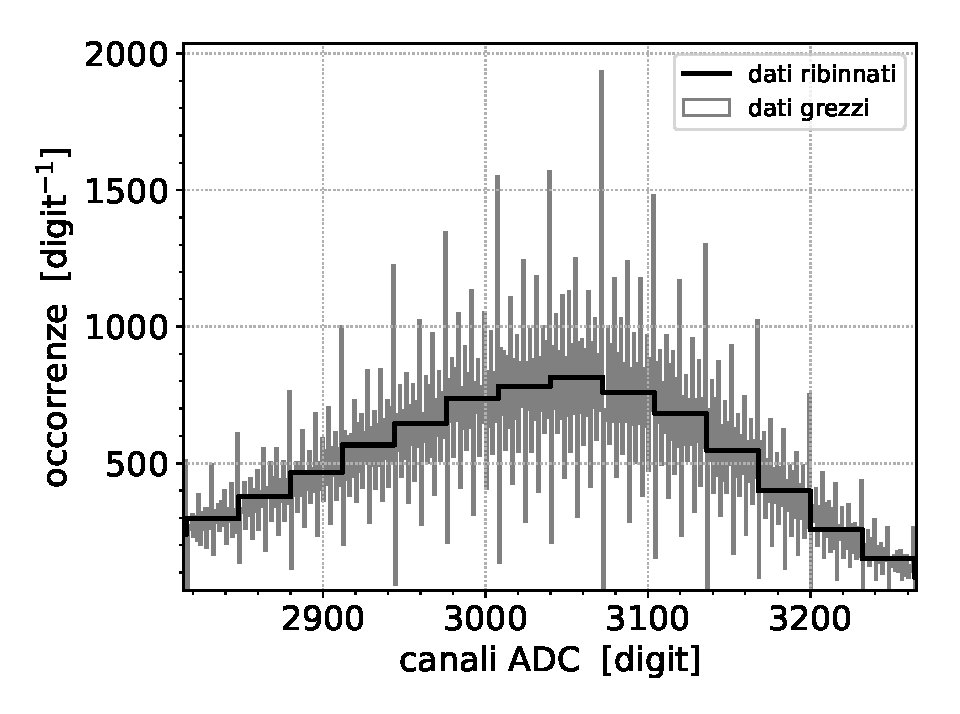
\includegraphics[width=25 em]{immagini/rebin}
\caption{Istogramma di una parte dei dati della misura di stabilità in cui si vedono gli accumuli a cui è soggetta l'ADC e la nostra soluzione.}
\label{picchi}
\end{figure}

\paragraph{Guadagno dell'amplificatore}

Abbiamo verificato se la risposta dello spettrometro dipende come atteso dal guadagno dell'amplificatore
e abbiamo notato un comportamento inatteso dell'apparato.
Variando il guadagno dell'amplificatore agendo sulla manopola \texttt{coarse}
osserviamo gli spettri riportati in \autoref{fig:guadagno}.
La forma dello spettro non varia con un semplice fattore moltiplicativo:
la larghezza del picco è circa uguale per un guadagno di 25 e 100
e la posizione del picco non è quella attesa.
Questa dipendenza incompresa della forma dello spettro da questo parametro
non ci permette di trovare un modello fisico per la stessa.

\begin{figure}[h]
	\centering
	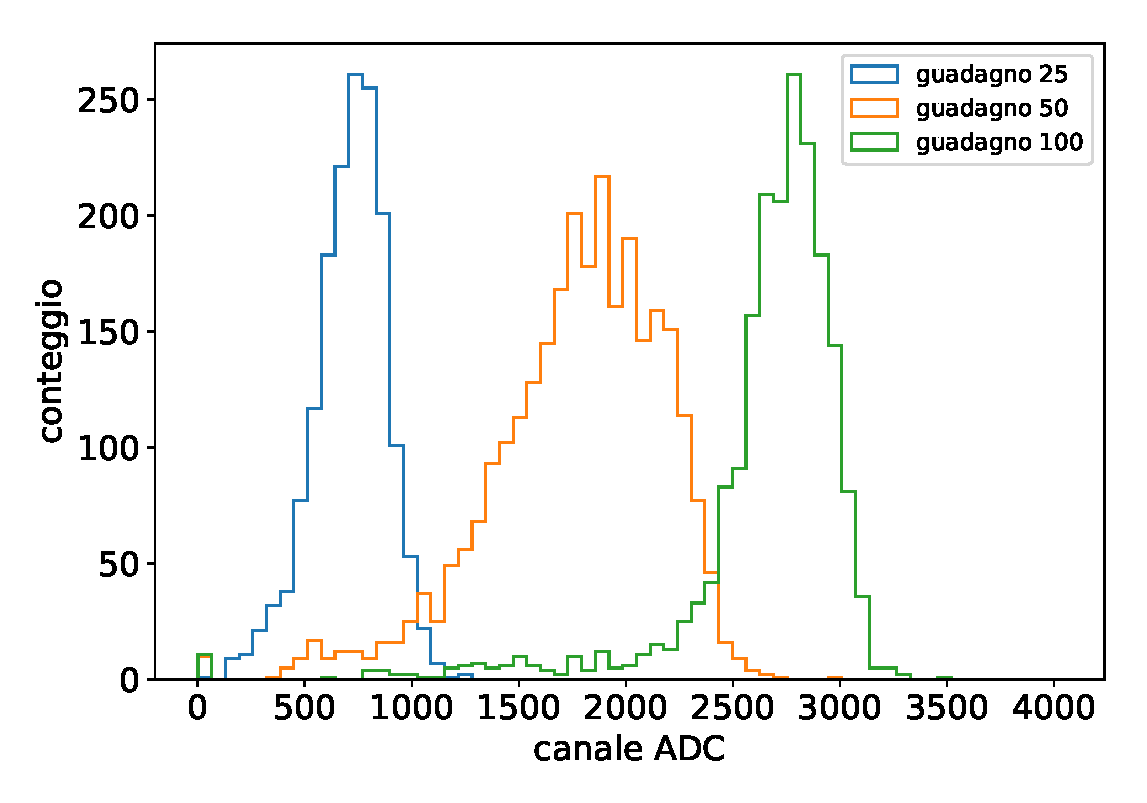
\includegraphics[width=30 em]{immagini/all8}
	\caption{Risposta dello spettrometro al variare del guadagno dell'amplificatore. Gli spettri non variano come atteso.}
	\label{fig:guadagno}
\end{figure}